\documentclass{article}

\usepackage{amsmath}
\usepackage{graphicx}

\DeclareMathOperator{\Argmax}{argmax}
\newcommand{\PosC}{\mathrm{Pos}}
\newcommand{\NegC}{\mathrm{Neg}}

\title{Na\"{i}ve Bayes Classifier for Sentiment}
\author{James Cook, Reynold Xin}

\date{2012-02-07}

\begin{document}
	
\maketitle

\section{The Problem}
We design an algorithm to solve the following problem. Given a document, we classify the sentiment of the document as either positive or negative. This problem is known as binary sentiment analysis and has broad applications. For example, it can be used to understand the customer feedback for a particular product automatically without manually reading all the reviews. In this particular assignment, we are tasked with sentiment analysis for movie reviews.


\section{Method}

\subsection{Classifier Model}

We use a na\"ive Bayes model, in which the documents are generated according to the following process.
First, a class \(c\) is chosen from a probability distribution \(\Pr(c)\).
Then, a document from class \(c\) is generated.
We tried a multinomial model and a Bernoulli model to model this process.
\begin{itemize}
\item \emph{Multinomial model.}  A document length \(m_d\) is chosen and \(m_d\) words \(w_{d,1}, \dotsc, w_{d,m_d}\) are chosen independently from a distribution \(\Pr(w|c)\).
\item \emph{Bernoulli model.}  For each word \(w\) in the vocabulary, \(w\) is added to the document with probability \(\Pr(w|c)\).
\end{itemize}
The distributions \(\Pr(c)\) and \(\Pr(w|c)\) are parameters of the model.

\subsection{Document Representation}

We represent each document \(d\) as a list of words \(w_{d,1}, \dotsc, w_{d,m_d}\).
In the simplest case, \(w_{d,i}\) was equal to the \(i\)-th token of the document as it appeared in the data set.
This is an appropriate representation when using the multinomial model of document generation.
When using the Bernoulli model, we removed duplicate occurrences of words.

We tried using the Porter stemming algorithm.
Stemming is the process of reducing inflected and derived words to their stem \cite{porter-stemmer}.
Word \(w_{d,i}\) in our document representation is then the result of applying the stemming function to the \(i\)-th word of the document as it appeared in the input data set.
Stemming incidentally reduces the number of features used in the classifier.
For example, using the Porter Stemmer \cite{porter-stemmer}, both ``apply'' and ``applying'' become the same stem ``appli''.

In all, we tried four different document representations: multinomial and Bernoulli, together with not-stemmed words and word stems.
In Section~\ref{sec:EvalAndTuning}, we explain how we chose among these four possibilities.

\subsection{Training and Classification}

Using the na\"ive Bayes classifier, for a class \(c \in \{\PosC, \NegC\}\) and document \(d\) consisting of words \(w_{d,1},\dotsc,w_{d,m_d}\) (where each word occurs at most once in the Bernoulli version), we have
\[\Pr(c|d)=\frac{\Pr(d|c)\Pr(c)}{\Pr(d)}\]
where
\[\Pr(d|c)=\sum_{i=1}^{m_d}\Pr(w_i|c)\ldotp\]
Our training procedure sets \(\Pr(c)\) to be the fraction of documents with class \(c\),%
\footnote{After inspecting the data set, we found this ratio to be \(1/2\).  Setting \(P(c)\) to \(1/2\) is equivalent to dropping the term, so we ignored it in our implementation.}
and sets
\[\Pr(w|c)=\frac{n_{w,c}+\alpha}{\sum_{w'}(n_{w',c}+\alpha)}\ldotp\]
When testing, our model classifies a document \(d\) as \(\Argmax_c\Pr(c|d)\).

\(\alpha\) is a parameter of the model.
Setting \(\alpha=0\), training would maximumize the likelihood of the data given the parameters.
Unfortunately, the maximum likelihood parameters set \(\Pr(d|c)=0\) whenever document \(d\) contains a word that never occurred in class \(c\) in the training data.
It is desirable to allow some new uses of words in new documents, so we set \(\alpha\) to be a positive number.
We explain how we choose the value of \(\alpha\) in next section.


\section{Experiments}
\label{sec:Results}


\subsection{Evaluation Methodology}

We implemented our Na\"{i}ve Bayes sentiment classifier in Scala 2.9.1 and tested the classifier on the polarity movie review dataset \cite{polarity-dataset, Pang+Lee:04a}. The dataset contains 1000 documents labeled as ``favorable'' and 1000 documents labeled as ``disfavorable''.
\footnote{To avoid confusion, we will refer to positive reviews as ``favorable'' and negative reviews as ``disfavorable'' in this section.}

We chose evaluate the model's performance on a testing set using the \(F_1\) score.  The \(F_1\) score is defined as:
\[
  F_1=
  \frac
      {2\cdot\#\text{true positive}}
      {2\cdot\#\text{true positive}+\#\text{false negative}+\#\text{false positive}}
  \ldotp
\]
We had some difficulty interpreting this in the context of a classification task.
We decided that the score makes sense when focusing on a particular label.
For example, if we are interested in the model's performance with the label ``favorable'', then we count test results as follows.

\begin{tabular}{c|c|c}
  true class & model classification & interpretation for ``favorable'' \\
  \hline
  favorable & favorable & true positive \\
  favorable & disfavorable & false negative \\
  disfavorable & favorable & false positive \\
  disfavorable & disfavorable & true negative \\
\end{tabular}

We define the resulting F1 model score to be \(F_1(\PosC)\).
We define \(F_1(\NegC)\) the same way but with the roles of ``favorable'' and ``disfavorable'' reversed, and score the model as
\[\text{model score}=\tfrac12 (F_1(\PosC) + F_1(\NegC)) \ldotp\]

We had three parameters to tune: multinomial or Bernoulli; whether to stem words; and the smoothing parameter \(\alpha\).  We tried all combinations of the first two parameters, with \(\alpha\) varying between \(0.1\) and \(30\) with a ratio of \(\sqrt{2}\) between successive \(\alpha\)-values (\(0.1, 0.1\sqrt{2}, 0.2, 0.2\sqrt{2}, \dotsc\)).  Using a geometric series allowed us to try many ranges of size for the \(\alpha\) parameter; once we identified the range with the best performance, we did a second pass with a finer range of \(\alpha\)-values as explained in Section~\ref{sec:alpha}.

We used 10-fold cross-validation to evaluate the performance of our algorithm.  We chose a random order for the documents once, and for each parameter setting, we evaluated the model ten times (using successive slices as the held-out test set) and recorded the average score of the model on those ten sets.


\subsection{Parameter Tuning}
\label{sec:alpha}

Figure \ref{all-combo} shows the F1 scores for various combinations of parameters. The x\-axis varies the value for smoothing parameter \(\alpha\), and the y\-axis reports the F1 model score. From the graph, it is obvious that the best setup is using a multinomial model without stemming.

\begin{figure}
  \centering
  \caption{F1 measures for various combinations of parameters.}
  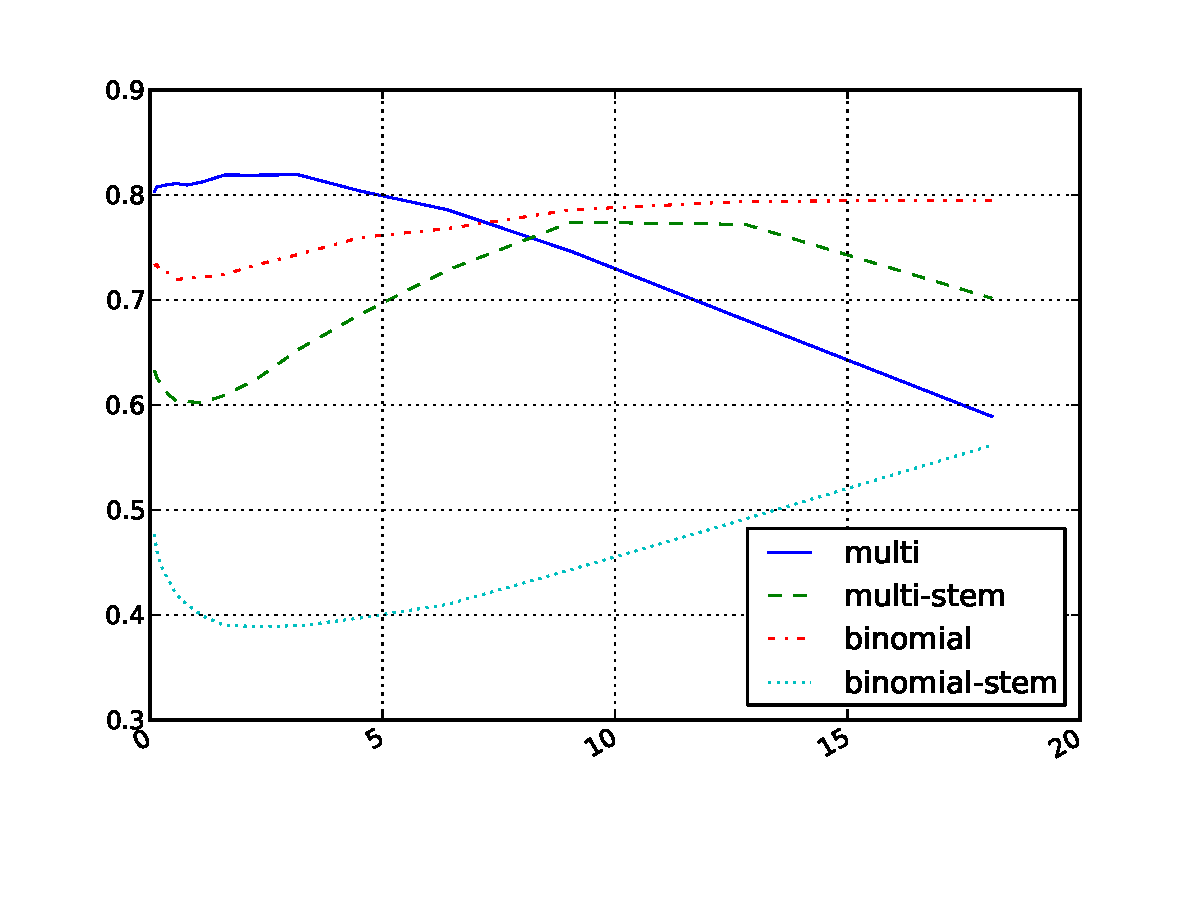
\includegraphics[width=0.9\textwidth]{graphs/all-combo.pdf}
  \label{all-combo}
\end{figure}

\begin{figure}
  \centering
  \caption{Tuning smoothing factor alpha.}
  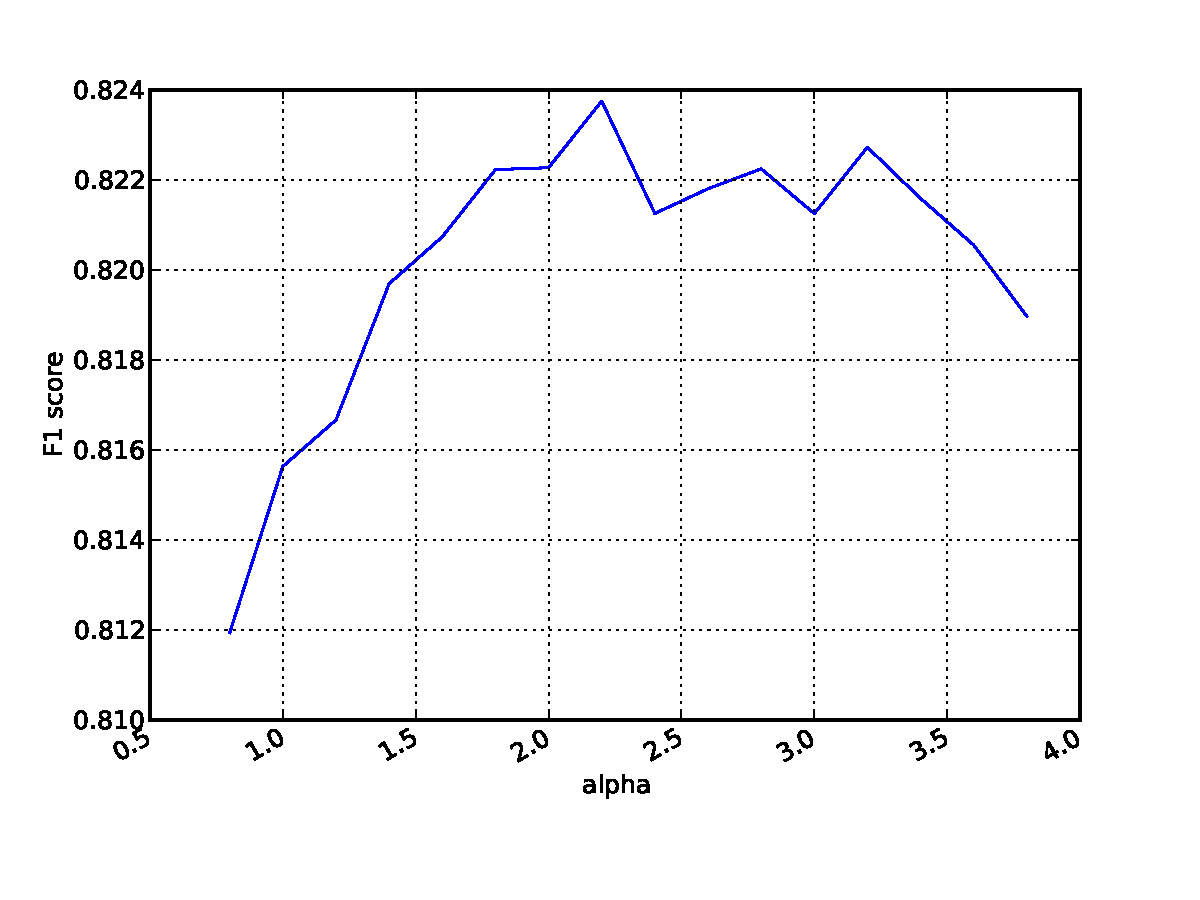
\includegraphics[width=0.9\textwidth]{graphs/alpha.pdf}
\end{figure}


\textbf{Stemming}: We observed that stemming the words had a negative impact on the F1 score for both multinomial or Bernoulli models, while using more computational resources. We speculate that the choices of variations of words indeed carry connotations on sentiments. This observation is consistent with findings from previous works \cite{stanford-tutorial, sentiment-twitter}.

\textbf{multinomial or Bernoulli}: We observed that multinomial models perform better than Bernoulli models. This is expected as movie reviews are long documents. Based on our understanding, multinomial models work better for longer documents, while Bernoulli models work better for very short documents.

Somewhat surprising is the result that when the smoothing parameter \(\alpha\) is large, Bernoulli models actually have reasonable model score. Smoothing parameter \(\alpha\) defines the weight for unobserved words. Having a large smoothing parameter effectively reduces the weight for rare, observed words.

\textbf{Smoothing parameter \(\alpha\)}: For the best model setup (i.e. multinomial without stemming), we trained our classifier using a finer range of \(\alpha\)-values, chosen between 0.6 to 3.8 with setup size 0.2. Assuming this is a convex function, we found the best range for \(\alpha\) is between 1.6 to 3.6. 


\subsection{Top Term Weights}
\label{sec:TopWords}

% Program output:
%(false,false,2.2,0.822)
%Pos: List((shrek,3.230), (mulan,3.138), (flynt,2.9035111177554587), (gattaca,2.8346396128564333), (ordell,2.759), (truman's,2.6187512324233975), (lebowski,2.6168669281160994), (guido,2.588), (leila,2.55661945131639), (sweetback,2.490))
%Neg: List((nbsp,-3.4045562750852802), (seagal,-3.1096499422617025), (brenner,-2.747), (sphere,-2.572643333537556), (schumacher,-2.556), (stigmata,-2.493), (1900,-2.451), (pokemon,-2.406976211648738), (bye,-2.406976211648738), (jawbreaker,-2.404))
%Pos (mf): List((,,6988.590), (the,5680.522), (and,5062.829), (is,3480.295), (of,3031.905), (his,2302.1047630517264), (as,2103.495762997044), (he,1394.452), (in,1206.934), (a,976.3928793058776))
%Neg (mf): List((.,-3176.335), (",-2935.369), (i,-1874.9698007890427), (movie,-1832.499865514896), (?,-1631.999), (bad,-1574.092), (this,-1474.2238454822032), (have,-1308.290), (!,-974.078), (no,-939.664))

To better understand the behavior of our algorithm, we made a list of the words \(w\) with the ten highest and ten lowest values \(\Pr(\PosC|w)\).
We used our best set of model parameters: multinomial model; no stemming; \(\alpha=2.2\).
Figure~\ref{fig:HighestWeightWords} lists these words, together with the log ratio \(\log(\Pr(\PosC|w) / \Pr(\NegC|w))\) (which is a monotone function of \(\Pr(\PosC|w)\)).
We observe that the list seems to consist of uncommon words.
This is not surprising: if a word appears exclusively in one class of document, then our model will infer that the word is much more likely to come from that class, even if the total number of occurrences is relatively small (as long as the number of occurrences is larger than the smoothing parameter \(\alpha\)).

\begin{figure}
\begin{tabular}{c|c}
    \multicolumn{2}{c}{Words most likely to be positive} \\
    word & \(\log(\Pr(\PosC|w) / \Pr(\NegC|w))\) \\
    \hline
    shrek & 3.230 \\
    mulan & 3.138 \\
    flynt & 2.904 \\
    gattaca & 2.835 \\
    ordell & 2.759 \\
    truman's & 2.619 \\
    lebowski & 2.617 \\
    guido & 2.588 \\
    leila & 2.557 \\
    sweetback & 2.490
\end{tabular}
\begin{tabular}{c|c}
    \multicolumn{2}{c}{Words most likely to be negative} \\
    word & \(\log(\Pr(\PosC|w) / \Pr(\NegC|w))\) \\
    \hline
    nbsp & -3.405 \\
    seagal & -3.110 \\
    brenner & -2.747 \\
    sphere & -2.573 \\
    schumacher & -2.556 \\
    stigmata & -2.493 \\
    1900 & -2.451 \\
    pokemon & -2.407 \\
    bye & -2.407 \\
    jawbreaker & -2.404
\end{tabular}
\caption{\label{fig:HighestWeightWords} Words most likely to come from positive or negative reviews}
\end{figure}

To better understand which words the model \emph{typically} finds useful in classifying documents, we made a second pair of lists, this time multiplying each word's weight by the number of occurrences of the word in the data set: so we sort words according to \(n_w \cdot \log(\Pr(\PosC|w) / \Pr(\NegC|w))\), where \(n_w\) is the number of occurrences of the word in the data set.
The resulting lists are shown in Figure~\ref{fig:MostInfluentialWords}.
These lists contain many common words and punctuation marks that we would not have thought were associated with negative or positive sentiments.

There is reason to believe these words did have a strong effect on the performance of our classifier.
If for each word \(w\) we define \(s_w = \log(\Pr(\PosC|w_{d,i}) / \Pr(\PosC|w_{d,i}))\), then
our classification algorithm for a document \(d\) is equivalent to computing \(\sum_{i=1}^{m_d} s_w\) and choosing \(\PosC\) or \(\NegC\) if the sum is positive or netagive.
A word with a high value of \(n_w \cdot s_w\) can be thought of as having a great influence over these sums.
We therefore find it concerning that words like ``the'' and ``and'', and simple punctuation marks, score so highly.
It is possible that these are indeed useful indicators for positve or negative sentiment, but just in case, in future work it is worth trying a version of the algorithm that excludes common tokens.

\begin{figure}
\begin{tabular}{c|c}
    \multicolumn{2}{c}{Most influential positive words} \\
    word & \(n_w \cdot \log(\Pr(\PosC|w) / \Pr(\NegC|w))\) \\
    \hline
     , & 6989 \\
    the & 5681 \\
    and & 5063 \\
    is & 3480 \\
    of & 3032 \\
    his & 2302 \\
    as & 2103 \\
    he & 1394 \\
    in & 1207 \\
    a & 976.4
\end{tabular}
\begin{tabular}{c|c}
    \multicolumn{2}{c}{Most influential negative words} \\
    word & \(n_w \cdot \log(\Pr(\PosC|w) / \Pr(\NegC|w))\) \\
    \hline
    . & -3176 \\
    " & -2935 \\
    i & -1875 \\
    movie & -1832 \\
    ? & -1632 \\
    bad & -1574 \\
    this & -1474 \\
    have & -1308 \\
    ! & -974.1 \\
    no & -939.7
\end{tabular}
\caption{\label{fig:MostInfluentialWords} Words with much total influnce on our classifier (see Section~\ref{sec:TopWords}).}
\end{figure}


\section{Conclusion}
We designed and implemented a Na\"{i}ve Bayes sentiment analysis classifier. Using a movie review dataset, we tested four different setups for the sentiment classifier and concluded that the best setup is using a multinomial model without stemming. We also tested different values for the smoothing parameter and found the best smoothing value to be between 1.6 and 2.6.


\bibliography{report}{}
\bibliographystyle{plain}

\end{document}
